\documentclass[10pt,a4paper]{article}
\usepackage[utf8]{inputenc}
\usepackage[german]{babel}
\usepackage{mathrsfs}
\usepackage{amsmath}
\usepackage{amsfonts}
\usepackage{amssymb}
\usepackage{amsthm}
\usepackage{minted}
\usepackage{graphicx}
\usepackage[left=2cm,right=2cm,top=2cm,bottom=2cm]{geometry}

\begin{document}

\section{Aufgabe 1}

\subsection{Teil a}

\subsubsection{i)}

The hyperparameters are optimized in the following cell
\begin{minted}{julia}
using Optim
g(khp) = GP(m, k, khp)                # function that defines a GP (including hyperparameters)
f(hp)  = -logmarginallikelihood(g(hp[1:end-1]), hp[end]^2, D)   # define the objective function
hp0    = randn(nhp)                  # random starting point
res    = optimize(f, hp0)            # find the minimum
hp     = res.minimum                 # the optimal hyperparameter
\end{minted}
Here $f$ is the negative loglikelihood, that is then optimized with some
optimization algorithm and automatic forward differentiation with dual numbers.

\subsubsection{ii)}

\begin{minted}{julia}
dot(x', A \ x)
\end{minted}

\subsubsection{iii)}

\begin{minted}{julia}
chol(Sigma, :L) * randn(d) + mu
\end{minted}
We set the optional argument \mintinline{julia}{:L}, because
\mintinline{julia}{chol} returns a upper triangular matrix by default, but we
need a lower one, so that $LL^T = \Sigma$ instead of $R^TR = \Sigma$.

\begin{proof}
  Let $\Sigma$ a positive definite $d \times d$-matrix, $\Gamma$ its Cholesky
  decomposition, $m$ a $d$-dimensional vector, $x \sim \mathcal{N}(0_d, I_d)$
  and $y = \Gamma \cdot x + \mu$. Then the probability density function of $y$
  is
  \begin{align*}
    p(y = z) & = p(\Gamma \cdot x + \mu = z)\\
             & = p(x = \Gamma^{-1} \cdot (z - \mu))\\
             & = \frac{1}{\sqrt{2 \pi}^d} \exp \left( -\frac{1}{2} (\Gamma^{-1} \cdot (z - \mu))^T I_d^{-1} (\Gamma^{-1} \cdot (z - \mu)) \right)\\
             & = \frac{1}{\sqrt{2 \pi}^d} \exp \left( -\frac{1}{2} (z - \mu)^T (\Gamma^{-1})^T \Gamma^{-1} (z - \mu) \right)\\
             & = \frac{1}{\sqrt{2 \pi}^d} \exp \left( -\frac{1}{2} (z - \mu)^T (\Gamma^T)^{-1} \Gamma^{-1} (z - \mu) \right)\\
             & = \frac{1}{\sqrt{2 \pi}^d} \exp \left( -\frac{1}{2} (z - \mu)^T (\Gamma\Gamma^T)^{-1} (z - \mu) \right)\\
             & = \frac{1}{\sqrt{2 \pi}^d} \exp \left( -\frac{1}{2} (z - \mu)^T \Sigma^{-1} (z - \mu) \right)\\
             & \propto \mathcal{N}(\mu, \Sigma)
  \end{align*}
  So $y \sim \mathcal{N}(\mu, \Sigma)$.
\end{proof}

\subsection{Teil b}

\subsubsection{Dataset 1}

Kernel
\begin{minted}{julia}
k(a, b, khp) = kse(a, b, khp[1:2]) + kper(a, b, khp[3:5]) * kse(a, b, khp[6:7])
\end{minted}
This maximizes the log-likelihood to infinity at
\begin{minted}{shell}
8-element Array{Float64,1}:
 -1.11567
  2.12066
  0.847791
 -0.789038
 -0.22991
 -1.46606
 -0.666645
 -0.00338305
\end{minted}
and extrapolates with a super-low variance, but does not really match the
picture drawn by the data.
\begin{figure}[h]
  \centering
  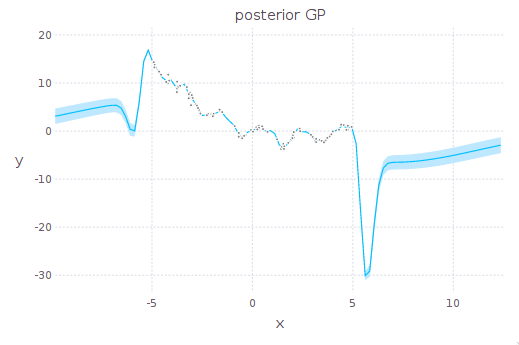
\includegraphics[width=350pt]{1_b_1}
  \caption{Suspiciously good fit for dataset \#1}
\end{figure}

\subsubsection{Dataset 2}

Here I used the kernel
\begin{minted}{julia}
k(a, b, khp) = kse(a, b, khp[1:2]) + kper(a, b, khp[3:5]) + kper(a, b, khp[6:8])
\end{minted}
with one squared exponentional for smoothness, one periodic kernel for short
cycles and one for long ones. The loglikelihood was once again optimized to
infinity. I think, there is something funny going on. But this time I like the
plot a lot.
\begin{figure}[h]
  \centering
  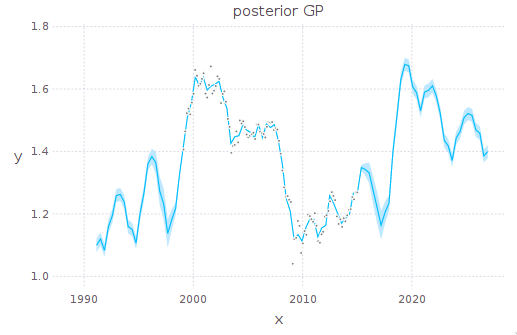
\includegraphics[width=350pt]{1_b_2}
  \caption{Prediction of exchange rates}
\end{figure}

\subsubsection{Dataset 3}

I just used the kernel from the book without the second squared exponentional.
\begin{minted}{julia}
k(a,b,khp) = kse(a,b,khp[1:2]) + krq(a,b,khp[3:5]) +
    kper(a, b, khp[6:8]) * kse(a, b, khp[9:10])
\end{minted}
After my failed attempt at parallel programming in julia I found through sheer
luck hyperparameters, that resulted in a loglikelihook of $54.7$.
\begin{figure}[h]
  \centering
  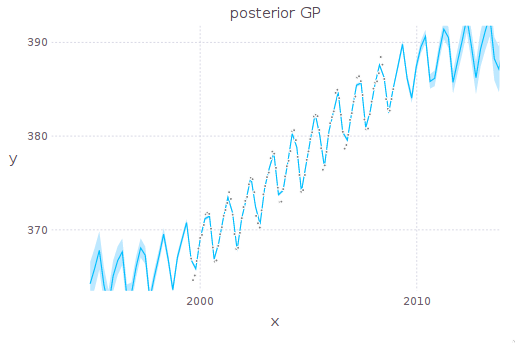
\includegraphics[width=350pt]{1_b_3}
  \caption{I probably used up my luck of the next two weeks for this}
\end{figure}

\section{Aufgabe 2}

\subsection{Teil a - d}

I downloaded the daily average temperature data for Düsseldorf from dwd.de and
computed the weekly means from it.
\begin{minted}{julia}
# Read CSV
file = "temperature.csv"
Draw = readdlm(file, ',', Float64, header=true)[1][:, 2]

weekly_means = [mean(Draw[i:min(i + 6, end)]) for i = 1:7:size(Draw, 1)]

# Extract weekly mean temperatures of the last 2 years
temps = float(weekly_means[end - 52 * 2:end])
D = Data(float([i for i = 1:size(temps, 1)])', temps)

# STEP 1: set mean and kernel function
M = mean(temps)
m(a) = M
k(a, b, khp) = kse(a, b, khp[1:2]) + krq(a, b, khp[3:5]) + kper(a, b, khp[6:8])

# STEP 2: set the number of hyperparameters appropriately (add one for the noise variance)
nhp = 9
\end{minted}
The marginal loglikelihood is $-264.1$ with posterior parameters of
\begin{minted}{shell}
8-element Array{Float64,1}:
  15.1818
 -42.1509
  -2.59493
  -0.932232
  -2.01851
  22.9307
  -2.16393
  -0.19354
\end{minted}
It took about ten optimization attempts for the GP to extrapolate the one-year
period. The other attempts extrapolated approximately linear functions with
large variance on both sides.
\begin{figure}[h]
  \centering
  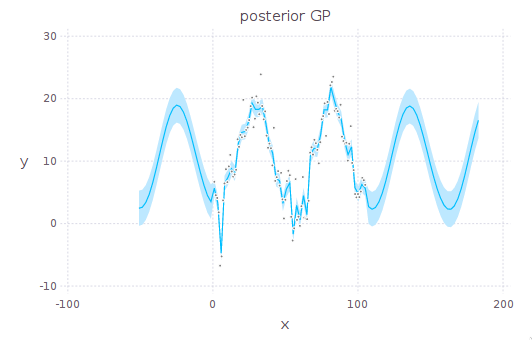
\includegraphics[width=350pt]{11_2}
  \caption{Weather data of Duesseldorf 2011-2012}
\end{figure}

\subsection{Teil e}

I chose this kernel function, because the weather data is obviously periodic and
points should be similar to points in their neighbourhood. The rational
quadratic kernel was added through experimentation, but I have no intuition
about it. I just did not work without it.

The output variance of both the SE and the periodic kernel is of the order of
20, which is about the difference between the minimum and maximum temperatures
over the course of a year.

It surprises me, that the inferred period of the periodic kernel is
$\simeq -0.2$, yet the extrapolation has periods of one year.

\end{document}